\documentclass[11pt]{report}

\usepackage{graphicx}
\usepackage{caption}

\marginparwidth 0.5in 
\oddsidemargin 0.25in 
\evensidemargin 0.25in 
\marginparsep 0.25in
\topmargin 0.0in 
\textwidth 6in \textheight 8.5in

\title{HW4: Use Cases}
\author{bolt1003}

\begin{document}
\maketitle

\chapter{Use Case Diagrams}
    \section{Project Management (bolt1003)}
        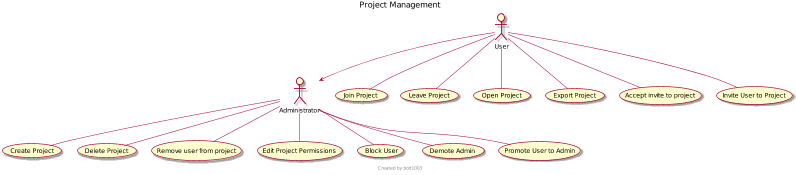
\includegraphics[width=\textwidth]{diagrams/usecase-projectmanagement}
        
\chapter{Sequence Diagrams}     
    \section{Compiler (bolt1003)}
        \begin{minipage}{1\textwidth}
            \begin{center}
                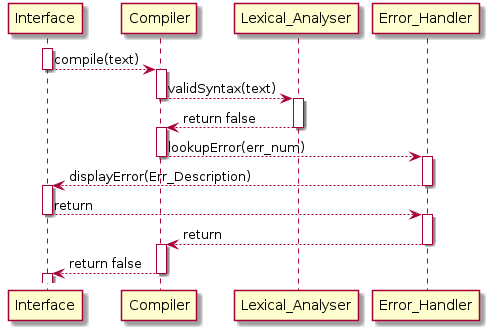
\includegraphics[width=0.7\textwidth]{diagrams/sequence-compiler}
            \end{center}
            \captionof{figure}{The sequence of a user attempting to compile a program with a syntax error.}
        \end{minipage}
        
\chapter{Class Diagrams}
\section{Project Management (bolt1003)}
    \begin{minipage}{1\textwidth}
        \begin{center}
            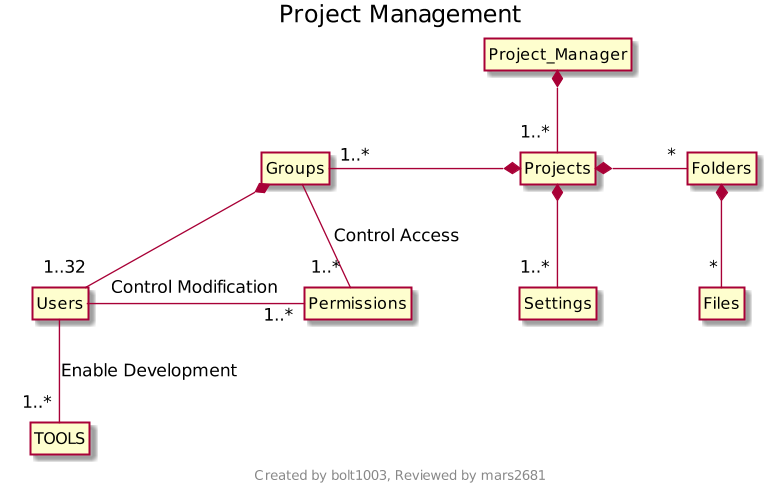
\includegraphics[width=0.9\textwidth]{diagrams/class-projectmanagement}
        \end{center}
        \captionof{figure}{Project management allows for the group to delicate permissions and create projects}
    \end{minipage}

\chapter{Requirements Documentation}

\section{Non-Functional Requirements}
    Non-functional requirements cover all the remaining requirements which are not covered by the functional requirements. They specify criteria that judge the operation of a system, rather than specific behaviours. Squire's non-functional requirements are:
    % Reliablity
    \begin{itemize}
         \item sQuire will leverage technology developed for the web to ensure reliablity. Technologies such as redunant hardware, redunant power providers, redunant internet services, load balancing and virtualization will enable sQuire to be reliable.(bolt1003)
     % Serviceability (bolt1003)
         \item sQuire will run in a virtual machine on top of redunant hardware. Using a virtual machine allows for mutliple instance to be running and tested. The backend will run on redunant hardware which will prevent hardware failure from affecting sQuire usage. In turn, allowing infrastructure to be serviced without affecting sQuire. (bolt1003)
    \end{itemize}

\section{Functional Requirements}
    Functional requirements will specify a behaviour or function. Squire's functional requirements are:
    
    \subsection{Communication (bolt1003)}
        \begin{itemize}
            \item Global text chat.
            \item Per project local chat.
            \item Private chat between users.
            \item A friends list with friend status icons and avatars.
            \item A global list of members in the project and status.
            \item Use of standard protocols such as XMPP or IRC.
            \item Third-party chat client access.
        \end{itemize}

\chapter{Application Domain Specification}

\section{Project Management (bolt1003)}
\subsection{Create Project}
\begin{tabular}{ p{2cm} p{12cm} }
 \hline
 \\
 \textit{Actors:} & Users of sQuire. \\ 
 \\
 \textit{Goals:} & Create a Project. \\
 \\
 \textit{Pre-conditions:} & The user is logged in and at the dashboard. \\
 \\
 \textit{Summary:} & The user creates a project. \\ 
 \\
 \textit{Related use cases:} & None. \\ 
 \\
 \textit{Steps:} & \begin{enumerate}
  \item User selects the "+" icon and a wizard appears.
  \item A name is choosen for the project.
  \item Language is selected from a drop down menu.
  \item User clicks finish.
 \end{enumerate} \\
 \\
 \textit{Alternatives:} & Create project from the editor. \\
 \\
 \textit{Post-conditions:} & The user assigns permissions to access the project. \\
 \\
\hline
\end{tabular}

\subsection{Open a project}
\begin{tabular}{ p{2cm} p{12cm} }
 \hline
 \\
 \textit{Actors:} & Users of sQuire. \\ 
 \\
 \textit{Goals:} & Choose the desired project and open it. \\
 \\
 \textit{Pre-conditions:} & One or more projects are available, the user is logged in and at the dashboard. \\
 \\
 \textit{Summary:} & User looks through a list of projects and selects the desired project. \\ 
 \\
 \textit{Related use cases:} & None. \\ 
 \\
 \textit{Steps:} & \begin{enumerate}
  \item User clicks on projects in the menu bar.
  \item A list of projects appears and the user clicks on the desired project.
 \end{enumerate} \\
 \\
 \textit{Alternatives:} & Open a project from recent projects. \\
 \\
 \textit{Post-conditions:} & User closes sQuire. \\
 \\
\hline
\end{tabular}

\subsection{Join Project}
\begin{tabular}{ p{2cm} p{12cm} }
\hline
\\
\textit{Actors:} & Users of sQuire. \\ 
\\
\textit{Goals:} & Join an existing project.\\
\\
\textit{Pre-conditions:} & Must be registered, logged in and have permission to join a project.\\
\\
\textit{Summary:} & The user logs in, chooses a project, and joins the project. \\
\\
\textit{Related use cases:} & Invite user to project, Accept user invite. \\
\\
\textit{Steps:} & \begin{enumerate}
 \item The user selects a project.
 \item The user chooses the "Join". 
 \item The project is added to the users projects bar.
 \item The user selects the project and selects "open".
\end{enumerate}\\
\\
\textit{Alternatives:} & User may decline an inventation to join a project. \\
\\
\textit{Post-conditions:} & None \\
\\
\hline
\end{tabular}

\subsection{Leave project}
\begin{tabular}{ p{2cm} p{12cm} }
 \hline
 \\
 \textit{Actors:} & User \\ 
 \\
 \textit{Goals:} & Remove member status from project. \\
 \\
 \textit{Pre-conditions:} & Logged in, member of the respective project, not project owner.  \\
\\
 \textit{Summary:} & A member of a project can unjoin that project at any time as long as they are not the project owner. To prevent mistakenly unjoining a project, the user is asked to confirm their decision.\\ 
 \\
 \textit{Related use cases:} & \\ 
 \\
 \textit{Steps:} & \begin{enumerate}
  \item User selects a project.
  \item User clicks "Unjoin". 
  \item User is promted to confirm their decision
  \item User clicks "Confirm".
  \item User is removed from project member list.    
 \end{enumerate} \\
 \\
 \textit{Alternatives:} & User clicks "Cancel" at step 4, in which case the task is ends at that point. \\
 \\
 \textit{Post-conditions:} & None. \\
 \\
\hline
\end{tabular}

\subsection{Delete Project}
\begin{tabular}{ p{2cm} p{12cm} }
\hline
\\
\textit{Actors:} & Users of sQuire.\\
\\
\textit{Goals:} & Delete an existing project. \\
\\
\textit{Pre-conditions:} & The user has the appropriate permissions to delete project. 
\\
\textit{Summary:} & A user deletes a project from the project workspace.\\
\\
\textit{Related use cases:} & Create a project. \\
\\
\textit{Steps:} & \begin{enumerate}
 \item The user selects a project.
 \item The user clicks on the "Delete project" button. 
 \item A dialog is displayed. 
 \item User select "delete" to delete the project. 
 \end{enumerate}\\
 \\
 \textit{Alternatives:} & User may choose not to delete the project in the confirmation display.\\
 \\
 \textit{Post-conditions:} & None. \\
 \\
\hline
\end{tabular}

\subsection{Export Project}
\begin{tabular}{ p{2cm} p{12cm} }
\hline
\\
\textit{Actors:} & User of sQuire.\\
\\
\textit{Goals:} & Export a workspace to a local file. \\
\\
\textit{Pre-conditions:} & The user needs permission to export the project. 
\\
\textit{Summary:} & User saves a file containing the project settings and files to a local machine. \\
\\
\textit{Related use cases:} & Importing a project, Creating a new project. \\
\\
\textit{Steps:} & \begin{enumerate}
 \item The user clicks on the "Export File" button. 
 \item System prompts the user to select a location and filename. 
 \item User selects a file location.
 \item The user enters a file name.
 \item The user selects "export". 
 \end{enumerate}\\
 \\
 \textit{Alternatives:} & The user cancels the export, The system prompts that a file already exists with the same name.\\
 \\
 \textit{Post-conditions:} & None. \\
 \\
\hline
\end{tabular}

\subsection{Accept Invite to Project}
\begin{tabular}{ p{2cm} p{12cm} }   
 \hline
 \\
 \textit{Actors:} & User who received the invite. \\
 \\
 \textit{Goals:} & Gain access to a Project. \\
 \\
 \textit{Pre-conditions:} & User has a valid email address. \\
 \\
 \textit{Summary:} & Access is granted to a project using an invitation email. \\ 
 \\
 \textit{Related use cases:} & Create an account. \\
 \\
 \textit{Steps:} & \begin{enumerate}
  \item Invitee clicks on the link received by email.
	 \item The link opens in a browser.
	 \item Dialog appear welcoming them to the project.
	 \item The project is added to their Projects list.
	\end{enumerate} \\
 \\
 \textit{Alternatives:} & The user ignores the invite. \\
 \textit{Post-conditions:} & Email link is deactivated. \\
 \\
\hline
\end{tabular}

\subsection{Remove User from Project}
\begin{tabular}{ p{2cm} p{12cm} }   
 \hline
 \\
 \textit{Actors:} & User of sQuire \\
 \\
 \textit{Goals:} & Revoke access to the Project for a single or multuple users. \\
 \\
 \textit{Pre-conditions:} & The user has permission to edit the Project access list. \\
 \\
 \textit{Summary:} & One or more user accounts are removed from the access list for a project. \\ 
 \\
 \textit{Related use cases:} & Add users to a project.  \\ 
 \\
 \textit{Steps:} & \begin{enumerate}
  \item The user selects the access list for the project.
	 \item The user selects an account. 
	 \item The user selects "Remove from Project".
	 \item The user is prompted for confirmation
	 \item The user selects 'Yes'.
 \end{enumerate} \\
 \\
 \textit{Alternatives:} & The user selects 'No' and the access list is not modified. \\
 \\
 \textit{Post-conditions:} &
    \begin{itemize}
	 \item The user that was removed is notified of the change.
	 \item The user is prevented from accessing files.
    \end{itemize}\\
 \\
\hline
\end{tabular}

\subsection{Edit Project Permissions}
\begin{tabular}{ p{2cm} p{12cm} }
 \hline
 \\
 \textit{Actors:} & User of sQuire \\ 
 \\
 \textit{Goals:} & Edit the permissions for a project \\
 \\
 \textit{Pre-conditions:} & The user is logged in. \\
 \\
 \textit{Summary:} & User opens up the settings menu and navigates to permissions, adds (or removes) users individual access rights to the project.  \\ 
 \\
 \textit{Related use cases:} & Add user to project, Remove user from project. \\ 
 \\
 \textit{Steps:} & \begin{enumerate}
  \item The user selects a project.
  \item The user selects settings.
  \item The user selects permissions.
  \item The user selects user from list of users.
  \item The user adds read or write permissions to user.
  \item The user selects save to save changes.
  \item The user exits settings.
 \end{enumerate} \\
 \\
 \textit{Alternatives:} & User can remove read or write permission instead in step 6. User can discard changes instead in step 7. \\
 \\
 \textit{Post-conditions:} & None. \\
 \\
\hline
\end{tabular}

\subsection{Modify read/write access}
\begin{tabular}{ p{2cm} p{12cm} }
 \hline
 \\
 \textit{Actors:} & User \\ 
 \\
 \textit{Goals:} & Modify a user\'s permissions. \\
 \\
 \textit{Pre-conditions:} & User is signed in and holds Admin rights for the currently selected Project\\
 \\
 \textit{Summary:} & User modifies another User\'s read/write permissions to portions of the project. \\
 \\
 \textit{Related use cases:} & None. \\ 
 \\
 \textit{Steps:} & \begin{enumerate}
  \item User clicks Permissions Management
  \item System displays permissions management window
  \item User selects a file, multiple files, directory or entirety of project and grants/revokes read/write access
  \item System modifes the target User\'s permissions and notifies them.
 \end{enumerate} \\
 \\
 \textit{Alternatives:} & 3. User selects cancel, System discards changes. \\
 \\
 \textit{Post-conditions:} & None. \\
 \\
\hline
\end{tabular}

\subsection{Remove User}
\begin{tabular}{ p{2cm} p{12cm} }
    \hline
    \\
    \textit{Actors:} & User \\ 
    \\
    \textit{Goals:} & Remove a user from project. \\
    \\
    \textit{Pre-conditions:} & User is signed in, in project with Admin rights, and is on User Management page\\
    \\
    \textit{Summary:} & User removes a selected user from the Project \\ 
    \\
    \textit{Related use cases:} & Invite User, Modify Read/Write Access \\ 
    \\
    \textit{Steps:} & \begin{enumerate}
        \item User clicks Remove User button.
        \item System displays list of active users for project.
        \item User selects one or more other users from the list and presses Remove.
        \item System prompts User for verification.
        \item User presses Confirm.
        \item System removes the selected users from the project.
        \item System revokes read and write access from the selected users.
        \item System notifies selected users that they have been removed from the project.
    \end{enumerate} \\
    \\
    \textit{Alternatives:} & User presses Cancel in steps 3 or 5, System returns user to User Management page \\
    \\
    \textit{Post-conditions:} & None. \\
    \\
    \hline
\end{tabular}

\subsection{Invite User to Project}
\begin{tabular}{ p{2cm} p{12cm} }
    \hline
    \\
    \textit{Actors:} & User \\ 
    \\
    \textit{Goals:} & Invite user(s) to project \\
    \\
    \textit{Pre-conditions:} & User is signed in, in project with Admin rights, and is on User Management page \\
    \\
    \textit{Summary:} & User invites user(s) to the current project. \\ 
    \\
    \textit{Related use cases:} & Remove User, Join Project \\ 
    \\
    \textit{Steps:} & \begin{enumerate}
        \item User clicks Invite Users button
        \item System prompts user to enter username(s)/email(s)
        \item User enters username(s)/email(s) of the user(s) to invite and presses Ok.
        \item System looks up the specified user(s) and notifies them of invitation to the Project
    \end{enumerate} \\
    \\
    \textit{Alternatives:} & \begin{enumerate}
        \item User presses cancel in step 3, System returns User to User Management page
        \item In step 4, username(s)/email(s) don\'t match any users, System notifies User of failed invitiations.
    \end{enumerate} 
    \\
    \textit{Post-conditions:} & None. \\
    \\
    \hline
\end{tabular}

\subsection{Promote User to Admin}
\begin{tabular}{ p{2cm} p{12cm} }
    \hline
    \\
    \textit{Actors:} & User \\ 
    \\
    \textit{Goals:} & Promote a specified User to Admin \\
    \\
    \textit{Pre-conditions:} & User is signed in, in project with Admin rights, and is on User Management page \\
    \\
    \textit{Summary:} & User selects another User to be given Admin rights for the project. \\ 
    \\
    \textit{Related use cases:} & Demote Admin \\ 
    \\
    \textit{Steps:} & \begin{enumerate}
        \item User selects Promote to Admin.
        \item System displays a list of non-Admin active users.
        \item User selects user(s) and presses Submit.
        \item System prompts user for confirmation.
        \item User selects Confirm.
        \item System grants Admin permissions to the selected user(s).
    \end{enumerate} \\
    \\
    \textit{Alternatives:} & User presses cancel in steps 3 or 5, no action taken. \\
    \\
    \textit{Post-conditions:} & None. \\
    \\
    \hline
\end{tabular}

\subsection{Demote Admin}
\begin{tabular}{ p{2cm} p{12cm} }
    \hline
    \\
    \textit{Actors:} & User \\ 
    \\
    \textit{Goals:} & Demote Admin to user \\
    \\
    \textit{Pre-conditions:} & User is signed in, in project with Admin rights, and is on User Management page \\
    \\
    \textit{Summary:} & User demotes selected Admins to normal Users for the project. \\ 
    \\
    \textit{Related use cases:} & Promote User to Admin \\ 
    \\
    \textit{Steps:} & \begin{enumerate}
        \item User selects Demote Admin
        \item System displays list of Admins
        \item User selects Admin(s) to demote and presses Submit.
        \item System prompts User for confirmation.
        \item User presses Confirm.
        \item System revokes Admin rights from selected User(s)
    \end{enumerate} \\
    \\
    \textit{Alternatives:} & \begin{enumerate}
        \item User presses cancel in steps 3 or 5, no action taken
        \item User attempts to demote Admin that is the Owner of the project, System rejects request and notifies User.
    \end{enumerate}
    \\
    \textit{Post-conditions:} & None. \\
    \\
    \hline
\end{tabular}

\subsection{Block User}
\begin{tabular}{ p{2cm} p{12cm} }
    \hline
    \\
    \textit{Actors:} & User \\ 
    \\
    \textit{Goals:} & Block a user from the project \\
    \\
    \textit{Pre-conditions:} & User is signed in, in project with Admin rights, and is on User Management page \\
    \\
    \textit{Summary:} & User blocks a user from the project, making them unable to view the project. \\ 
    \\
    \textit{Related use cases:} & Demote Admin \\ 
    \\
    \textit{Steps:} & \begin{enumerate}
        \item User clicks Block User.
        \item System displays a list of active users.
        \item User selects other user(s) to block and presses Submit.
        \item System prompts User for confirmation.
        \item User presses Confirm.
        \item System blocks selected user(s) from the project, revoking read/write access, and revoking Admin status as necessary.
    \end{enumerate} \\
    \\
    \textit{Alternatives:} & User presses cancel in steps 3 or 5.
    \\
    \textit{Post-conditions:} & None. \\
    \\
    \hline
\end{tabular}

%##################################################################################################

\section{File Management (Created by snev7821, revised by bolt1003)}
\subsection{Add New File to Project (snev7821)}
\begin{tabular}{ p{2cm} p{12cm} }
\hline 
\\
 \textit{Actors:} & User of sQuire \\
 \\
 \textit{Summary:} & The user performs this task to add a new file to the project. \\
 \\
 \textit{Pre-conditions:} & \begin{enumerate}
  \item User must be registered.
  \item User must be logged in.
  \item User must have a project open.
 \end{enumerate} \\
 \\
 \textit{Steps:} & \begin{enumerate}
  \item User clicks File in the top menu bar.
  \item System opens a drop-down menu.
  \item User navigates to Add New File.
  \item System opens an Add New File dialog window.
  \item User selects the file type and names the file.
  \item User clicks Add.
  \item System adds the file to the project.
 \end{enumerate} \\
 \\
 \textit{Alternatives:} & \begin{enumerate}
  \item Step 1: The user right clicks in the project panel and the system continues on to step 2 above.
  \item Step 5: The user clicks Cancel and a new file is not added to the project.
 \end{enumerate} \\
 \\ 
 \textit{Post-conditions:} & \begin{enumerate}
  \item A new file is added to the project.
  \item The database is updated to reflect the changes.
 \end{enumerate} \\
 \\
 \textit{Related:} & Add Existing File to Project \\
 \\
\hline
\end{tabular} 
\newpage

\subsection{Add Existing File to Project (snev7821)}
\begin{tabular}{ p{2cm} p{12cm} }
\hline
 \\
 \textit{Actors:} & User of sQuire \\
	\\
	\textit{Summary:} & The user performs this task to add an existing file to the project. \\ 
	\\
	\textit{Pre-conditions:} & \begin{enumerate}
		\item User must be registered.
		\item User must be logged in.
		\item User must have a project open.
	\end{enumerate} \\
	\textit{Steps:} & \begin{enumerate}
		\item User clicks File in the top menu bar.
		\item System opens a drop-down menu.
		\item User navigates to Add Existing File.
		\item System opens an Add Existing File dialog window.
		\item User selects PC or SQuire or Github.
		\item System updates the dialog to reflect the selected source.
		\item User navigates to the file's location and selects it.
		\item User clicks Add.
		\item System adds the file to the project.
	\end{enumerate} \\
	\\
	\textit{Alternatives:} & \begin{enumerate}
		\item Step 1: The user right clicks in the project panel and the system continues on to step 2 above.
		\item Step 5-7: The user clicks Cancel and a new file is not added to the project.
	\end{enumerate} \\
	\\
	\textit{Post-conditions:} & \begin{enumerate}
		\item An existing file is added to the project.
		\item The database is updated to reflect the changes.
	\end{enumerate} \\
	\\
	\textit{Related:} & Add New File to Project \\
	\\
	\hline
\end{tabular}
\newpage

\subsection{Delete File (snev7821)}
\begin{tabular}{ p{2cm} p{12cm} }
\hline \\
	\textit{Actors:} & User of sQuire \\
	\\
	\textit{Summary:} & The user performs this task to delete a file from the project. \\
	\\
	\textit{Pre-conditions:} & \begin{enumerate}
		\item User must be registered.
		\item User must be logged in.
		\item User must have a project open.
		\item User must be administrator of project.
		\item Current project must have at least one file.
	\end{enumerate} \\
	\\
	\textit{Steps:} & \begin{enumerate}
		\item User right clicks a file in the project pane.
		\item System opens a drop-down menu.
		\item User navigates to \textit{Delete}.
		\item System opens an \textit{Delete File} dialog window, asking if the user is sure.
		\item User selects \textit{Yes}.
		\item System deletes the file from the project.
	\end{enumerate} \\
	\\
	\textit{Alternatives:} & \begin{enumerate}
		\item Step 5: The user clicks \textit{Cancel} instead and the file is not deleted from the project.
		\item The user selects multiple files before step 1.
	\end{enumerate} \\
	\\
	\textit{Post-conditions:} & \begin{enumerate}
		\item The file is deleted from the project.
		\item The database is updated to reflect the changes.
	\end{enumerate} \\
	\\
	\textit{Related:} & Delete Project \\
	\\
\hline
\end{tabular} 
\newpage


\subsection{Export Files (snev7821)}
\begin{tabular}{ p{2cm} p{12cm} }
\hline
	\\
	\textit{Actors:} & User of sQuire \\
	\\
	\textit{Summary:} & The user performs this task to download a number of files from a project. \\
	\\
	\textit{Pre-conditions:} &  \begin{enumerate}
		\item User must be registered.
		\item User must be logged in.
		\item User must have a project open.
		\item Must have at least one file in the project.
		\item User must have download permissions.
	\end{enumerate} \\
	\\
	\textit{Steps:} & \begin{enumerate}
		\item User clicks File in the top menu bar.
		\item System opens a drop-down menu.
		\item User navigates to Export Files.
		\item System opens an Export dialog window showing the project files on the left panel and the export location in the right panel.
		\item User selects a number of files on the left pane.
		\item User navigates to the export location in the right pane.
		\item User clicks Export.
		\item System downloads the selected files to the specified location.
	\end{enumerate} \\
	\\
	\textit{Alternatives:} & \begin{enumerate}
		\item Step 1: The user right clicks in the project panel and the system continues on to step 2 above.
		\item Step 5: User selects a folder and all files under that folder are selected.
		\item Step 5-6: The user clicks Cancel and the project is not exported.
	\end{enumerate} \\
	\\
	\textit{Related:} & Export Project \\
	\\
\hline
\end{tabular}
\newpage


\subsection{Open File in New Tab (snev7821)}
\begin{tabular}{ p{2cm} p{12cm} }
\hline
	\\
	\textit{Actors:} & User of sQuire \\
	\\
	\textit{Summary:} & Allows users to open a file. \\
	\\
	\textit{Goals:} & Opening files is essential in being able to work on a project. \\
	\\
	\textit{Pre-conditions:} &  \begin{enumerate}
		\item User is registered.
		\item User is logged in.
		\item User has a project open.
		\item Current project contains at least one file.
		\item User has read permission.
	\end{enumerate} \\
	\\
	\textit{Steps:} & \begin{enumerate}
		\item User double clicks a file.
		\item The editor opens its contents in a new tab and focuses on it.
	\end{enumerate} \\
	\\
	\textit{Alternatives:} & Step 1: Instead of double clicking a file, the user right clicks it and navigates to Open. \\
	\\
\hline
\end{tabular}
\newpage


\section{File Editing (snev7821)}
\subsection{View Line Numbers (snev7821)}
\begin{tabular}{ p{2cm} p{12cm} }
\hline
\\
	\textit{Actors:} & User of sQuire \\
	\\
	\textit{Summary:} & Allows the user to hide line numbers to the left of the document. \\
	\\
	\textit{Goals:} & In case user wants to hide line numbers so they have more space for text.\\
	\\
	\textit{Pre-conditions:} & \begin{enumerate}
		\item Must be registered.
		\item Must be logged in.
		\item User has view permission.
		\item A file is open.
		\item Line numbers are on
	\end{enumerate} \\
	\\
	\textit{Steps:} & \begin{enumerate}
		\item User selects the View menu option.
		\item System displays a drop-down with various options.
		\item User selects the Hide Line Numbers option.
		\item System hides line numbers to the left of the document.
	\end{enumerate} \\
	\\
	\textit{Related:} & \begin{enumerate}
		\item View References
		\item View Dates
		\item View Authors
	\end{enumerate} \\
	\\
\hline
\end{tabular}
\newpage


\subsection{View References (snev7821)}
\begin{tabular}{ p{2cm} p{12cm} }
\hline
\\
	\textit{Actors:} & User of sQuire \\
	\\
	\textit{Summary:} & Allows the user to view the number of references to a given function. \\
	\\
	\textit{Goals:} & It is useful to know the number of references to a given function for optimization and debugging purposes. \\
	\\
	\textit{Pre-conditions:} &  \begin{enumerate}
		\item Must be registered.
		\item Must be logged in.
		\item User has view permission.
		\item A \textit{code} file is open.
	\end{enumerate} \\
	\\
	\textit{Steps:} & \begin{enumerate}
		\item User selects the View menu option.
		\item System displays a drop-down with various options.
		\item User selects the View References option.
		\item System displays the number of references above each method declaration.
	\end{enumerate} \\
	\\
	\textit{Related:} & \begin{enumerate}
		\item Hide Line Numbers
		\item View Dates
		\item View Authors
	\end{enumerate} \\
	\\
\hline
\end{tabular}
\newpage


\subsection{View Dates (snev7821)}
\begin{tabular}{ p{2cm} p{12cm} }
\hline \\
	\textit{Actors:} & User of sQuire \\
	\\
	\textit{Summary:} & Allows the user to view the last date that each block of a document was edited. Blocks are defined as any number of lines that was written by a single user. Minimum block size is one line. \\
	\\
	\textit{Goals:} & This provides a useful metric for how up-to-date parts of the document are. \\
	\\
	\textit{Pre-conditions:} & \begin{enumerate}
		\item Must be registered.
		\item Must be logged in.
		\item User has view permission.
		\item A file is open.
	\end{enumerate} \\
	\\
	\textit{Steps:} & \begin{enumerate}
		\item User selects the View menu option.
		\item System displays a drop-down with various options.
		\item User selects the View Dates option.
		\item System displays the last date that each block of a document was edited.
	\end{enumerate} \\
	\\
	\textit{Related:} & \begin{enumerate}
		\item Hide Line Numbers
		\item View References
		\item View Authors
	\end{enumerate} \\
	\\
\hline
\end{tabular}
\newpage


\subsection{View Authors (snev7821)}
\begin{tabular}{ p{2cm} p{12cm} }
\hline
\\
	\textit{Actors:} & User of sQuire \\
	\\
	\textit{Summary:} & Allows the user to view the last author that edited each block of a document. Blocks are defined as any number of lines that was written by a single user. Minimum block size is one line. \\
	\\
	\textit{Goals:} & This is an accountability tool allowing other users to identify who is responsible for a change to a document. \\
	\\
	\textit{Pre-conditions:} & 
	\begin{enumerate}
		\item Must be registered.
		\item Must be logged in.
		\item User has read permission.
		\item A file is open.
	\end{enumerate} \\
	\\
	\textit{Steps:} & \begin{enumerate}
		\item User selects the View menu option.
		\item System displays a drop-down with various options.
		\item User selects the View Authors option.
		\item System displays the name of the last editor of each line of the document.
	\end{enumerate} \\
	\\
	\textit{Related:} & \begin{enumerate}
		\item Hide Line Numbers
		\item View References
		\item View Dates
	\end{enumerate} \\
	\\
\hline
\end{tabular}
\newpage


\subsection{Format Document  (snev7821)}
\begin{tabular}{ p{2cm} p{12cm} }
\hline \\
	\textit{Actors:} & User of sQuire \\
	\\
	\textit{Summary:} & Allows the user to format the document to a specified format \\
	\\
	\textit{Goals:} & An easy tool for making sweeping changes to a large part of a document. \\
	\\
	\textit{Pre-conditions:} & \begin{enumerate}
		\item Must be registered.
		\item Must be logged in.
		\item User has read/write permission.
		\item A file is open.
		\item The document has formatting options set.
	\end{enumerate} \\
	\\
	\textit{Steps:} & \begin{enumerate}
		\item User selects the Edit menu option.
		\item System displays a drop-down with various options.
		\item User selects the Format Document option.
		\item System formats the current document to the formatting settings currently set.
	\end{enumerate} \\
	\\
	\textit{Alternatives:} & \begin{enumerate}
		\item If no formatting settings are currently set, display a dialog box after step 3 and give the option for the user to do so now.
	\end{enumerate} \\
	\\
	\textit{Related:} & \begin{enumerate}
		\item Find/Replace
		\item Comment Section
	\end{enumerate} \\
	\\
\hline
\end{tabular}
\newpage


\subsection{Find/Replace  (snev7821)}
\begin{tabular}{ p{2cm} p{12cm} }
\hline
\\
	\textit{Actors:} & User of sQuire \\
	\\
	\textit{Summary:} &  Allows the user to find and/or replace phrases. \\
	\\
	\textit{Goals:} & This is a powerful tool that allows a user to make safer, quicker, and more efficient changes to a document. \\
	\\
	\textit{Pre-conditions:} &  \begin{enumerate}
		\item Must be registered.
		\item Must be logged in.
		\item User has read/write permission.
		\item A file is open.
	\end{enumerate}\\
	\\
	\textit{Steps:} & \begin{enumerate}
		\item User selects the Edit menu option.
		\item System displays a drop-down with various options.
		\item User selects the Find/Replace option.
		\item System displays a small form in an unobtrusive location.
		\item User enter the phrase to find and selects find.
		\item System highlights and focuses on the first occurrence of the phrase and all highlights all other occurrences.
	\end{enumerate} \\
	\\
	\textit{Alternatives:} & \begin{enumerate}
		\item User selects option to replace in step 5 and enters a phrase with which to replace the found occurrences of the searched phrase. The system replaces each occurrence.
	\end{enumerate} \\
	\\
	\textit{Related:} & \begin{enumerate}
		\item Format Document
		\item Find/Replace
	\end{enumerate} \\
	\\
\hline
\end{tabular}
\newpage


\subsection{Comment Section  (snev7821)}
\begin{tabular}{ p{2cm} p{12cm} }
\hline
\\
	\textit{Actors:} & User of sQuire \\
	\\
	\textit{Summary:} &  Allows the user to comment out a part of a document. \\
	\\
	\textit{Goals:} & A useful and quick way to disable a large part of a document. \\
	\\
	\textit{Pre-conditions:} & \begin{enumerate}
		\item Must be registered.
		\item Must be logged in.
		\item A file is open.
		\item User has read/write permission.
		\item Current open document supports commenting.
	\end{enumerate} \\
	\\
	\textit{Steps:} & \begin{enumerate}
		\item User selects the Edit menu option.
		\item System displays a drop-down with various options.
		\item User selects the Comment Section option.
		\item System comments the selected area.
	\end{enumerate} \\
	\\
	\textit{Alternatives:} & \begin{enumerate}
		\item If document does not support commenting, display a dialog box telling the user.
	\end{enumerate} \\
	\\
	\textit{Related:} & \begin{enumerate}
		\item Format Document
		\item Find/Replace
	\end{enumerate} \\
	\\
\hline
\end{tabular}
\newpage


\subsection{Display Typing User (snev7821)}
\begin{tabular}{ p{2cm} p{12cm} }
\hline \\
	\textit{Actors:} & User of sQuire \\
	\\
	\textit{Summary:} & As the user types, the system displays their name, their typing, and their caret, in a different color, to other users. \\
	\\
	\textit{Goals:} & Differentiate who is typing what. \\
	\\
	\textit{Pre-conditions:} & \begin{enumerate}
		\item Must be registered.
		\item Must be logged in.
		\item User has read/write permission.
		\item A file is open.
		\item Other users have the same document open.
	\end{enumerate} \\
	\\
	\textit{Steps:} & \begin{enumerate}
		\item User begins typing.
		\item System displays the user's typing, the user's name, and the user's caret, in a different color, to Other Users.
		\item Other Users see User typing, his username, and his caret, in a different color.
	\end{enumerate} \\
	\\
\hline
\end{tabular}
\newpage


\subsection{Display Syntax Highlighting  (snev7821)}
\begin{tabular}{ p{2cm} p{12cm} }
\hline
\\
	\textit{Actors:} & User of sQuire \\
	\\
	\textit{Summary:} &  As the user types code, the editor will change font color for different code structures and keywords. \\
	\\
	\textit{Goals:} & Aids the user is writing code and identifying key code parts. \\
	\\
	\textit{Pre-conditions:} & \begin{enumerate}
		\item Must be registered.
		\item Must be logged in.
		\item User has read/write permission.
		\item A supported code file is open.
	\end{enumerate} \\
	\\
	\textit{Steps:} & \begin{enumerate}
		\item User begins typing.
		\item System automatically colors special code structures and keywords.
	\end{enumerate} \\
	\\
	\textit{Related:} & Display Syntax Errors \\
	\\
\hline
\end{tabular}
\newpage


\section{User Prefrences (snev7821)}
\subsection{View User Preferences (snev7821)}
\begin{tabular}{ p{2cm} p{12cm} }
\hline
\\
    \textit{Actors:} & User of sQuire \\
	\\
	\textit{Summary:} & User views their preferences and from here can change them \\
	\\
	\textit{Goals:} & Allows user to view their preferences and change them \\
	\\
	\textit{Pre-conditions:} & \begin{enumerate}
		\item Must be registered
		\item Must be logged in
		\item User is on user homepage
	\end{enumerate} \\
	\\
	\textit{Steps:} & \begin{enumerate}
		\item User clicks "Manage Editor Preferences"
		\item System presents user with preferences page
	\end{enumerate} \\
	\\
	\textit{Related:} & Modify chat font, Modify chat color, Edit user color \\
	\\
\hline
\end{tabular}
\newpage


\subsection{Modify Chat Font (snev7821)}
\begin{tabular}{ p{2cm} p{12cm} }
\hline
\\
	\textit{Actors:} & User of sQuire \\
	\\
	\textit{Summary:} & User changes the chat font \\
	\\
	\textit{Goals:} & Allows user to change what chat font they see for themselves and others \\
	\\
	\textit{Pre-conditions:} & \begin{enumerate}
		\item Must be registered
		\item Must be logged in
		\item User is on user editor preferences page
	\end{enumerate} \\
	\\
	\textit{Steps:} & \begin{enumerate}
		\item User clicks "Modify Chat Fonts" button
		\item System brings up list of fonts, for the user and others
		\item User selects a font for self
		\item User sets a font for others
		\item System saves user choices after each user action
	\end{enumerate} \\
	\\
	\textit{Related:} & Modify chat color, Edit user editor theme \\
	\\
\hline
\end{tabular}
\newpage


\subsection{Modify Chat Color (snev7821)}
\begin{tabular}{ p{2cm} p{12cm} }
\hline
\\
	\textit{Actors:} & User of sQuire \\
	\\
	\textit{Summary:} & User changes the chat color \\
	\\
	\textit{Goals:} & Allows user to change what chat color they see for themselves and others \\
	\\
	\textit{Pre-conditions:} & \begin{enumerate}
		\item Must be registered
		\item Must be logged in
		\item User is on user editor preferences page
	\end{enumerate} \\
	\\
	\textit{Steps:} & \begin{enumerate}
		\item User clicks "Modify Chat Colors" button
		\item System brings up list of colors, for the user and others
		\item User selects a color for self
		\item User sets a color for others
		\item System saves user choices after each user action
	\end{enumerate} \\
	\\
	\textit{Related:} & Modify chat font, Edit user editor theme\\
	\\
\hline
\end{tabular}
\newpage


\subsection{Edit User Editor Theme (snev7821)}
\begin{tabular}{ p{2cm} p{12cm} }
\hline
	\\
	\textit{Actors:} & User of sQuire \\
	\\
	\textit{Summary:}User changes the Editor theme \\
	\\
	\textit{Goals:} & Allows user to change theme of the collaborative editor \\
	\\
	\textit{Pre-conditions:} & \begin{enumerate}
		\item Must be registered
		\item Must be logged in
		\item User is on user editor preferences page
	\end{enumerate} \\
	\\
	\textit{Steps:} & \begin{enumerate}
		\item User clicks "Modify Editor Theme" button
		\item System brings up list of themes for editor
		\item User selects a theme
		\item System saves user selection
	\end{enumerate} \\
	\\
	\textit{Related:} & Modify chat font, Edit user color \\
	\\
\hline
\end{tabular}
\newpage


\subsection{Turn Off Global Chat (snev7821)}
\begin{tabular}{ p{2cm} p{12cm} }
\hline
\\
	\textit{Actors:} & User of sQuire \\
	\\
	\textit{Summary:} & User turns off global chat \\
	\\
	\textit{Goals:} & Allows user to choose whether or not to engage in global chat \\
	\\
	\textit{Pre-conditions:} & \begin{enumerate}
		\item Must be registered
		\item Must be logged in
		\item User is on user editor preferences page
	\end{enumerate} \\
	\\
	\textit{Steps:} & \begin{enumerate}
		\item User checks "turn global chat off" box
		\item System brings up warning, explaining what this does
		\item User selects accept
		\item System saves user selection
		\item System disconnects user from global chat
	\end{enumerate} \\
	\\
	\textit{Related:} & Global chat \\
	\\
\hline
\end{tabular}
\newpage


\subsection{Psuedo-offline Mode (snev7821)}
\begin{tabular}{ p{2cm} p{12cm} }
\hline
\\
	\textit{Actors:} & User of sQuire \\
	\\
	\textit{Summary:} & User changes to offline mode \\
	\\
	\textit{Goals:} & Allows user to turn off online features, including chat, public profiles, etc. Site then serves as basic editing environment\\
	\\
	\textit{Pre-conditions:} & \begin{enumerate}
		\item Must be registered
		\item Must be logged in
		\item User is on user editor preferences page
	\end{enumerate}
	\\
\textit{Steps:} & \begin{enumerate}
		\item User clicks "offline mode" button
		\item System brings up warning
		\item User selects accept
		\item System saves user selection
		\item System closes chat
		\item System loads offline user page
		\item Upon disconnect with site, online mode restarts upon next connection
	\end{enumerate} \\
	\\
	\textit{Related:} & None \\
\hline
\end{tabular}
\newpage

\end{document}